\section{开源社区中的开放数据分析}

\subsection{数据的获取}
% GH Archive项目;
% Github事件日志、20种事件类型;
% ​更新周期:1周
\par 在世界范围内,开源开发人员同时在贡献着数百万个项目,为项目编写代码和文档、修复Bug、提交,而GH Archive 就是其中一个起到了记录作用的项目。它会记录公共的 GitHub 时间线,即按时间顺序录入GitHub 上所有行为活动的日志、存档,并使其能够被访问。本课题就使用了来自GH Archive的数据,开展进一步的研究。

\par 开源平台GitHub提供了 20 多种事件类型,范围从新的 Commit 和 Fork 事件,到提交新的 Pull Request、Comment 以及向项目添加成员。这些事件被聚合到每小时的存档中,自动更新,能够通过 HTTP 的方式访问获取。

\par 在本课题中,为了有效地进行开源项目或个人开发者的健康度衡量分析、呈现,在更新代价与数据有效性之间进行了折中选择,以1周为周期更新数据。

\subsection{数据预处理}
% 界定范围:Github全域;(还是仅活跃部分?)
% ​去除bot的极端数据
\par 为了能够更全面的了解开源社区的数据特征,同时保证其对当下情况较好的描述作用,在此选择了开源平台Github的2020年度全域数据作为样本,进行预处理以待进一步探索分析。

\par 在所有的数据中,由于Github Apps自动化协作机器人运行在服务端,可以同时服务于众多项目,从而具有了极高的活跃度和协作仓库数量,在后续统计开发者活跃度和活跃仓库数量时,对相关账号的协作行为进行了过滤。识别方法也很简单,即根据用户名后缀的[bot]进行账号识别。



\subsection{开放数据分析}
% 1. 全域开发者活跃情况:总体增长
% ​2. 开发者具有时区性:
% 3. 开发者使用语言分布:个人发展路径
% ​4. 项目中、项目间协作存在关系:开源进度不一,孤岛的存在,OpenGalaxy的评价标准(要放在这个部分吗?)
\par 从总体数据来看,2020 年全年的GitHub 全域事件日志数量总计约 8.6 亿条,较 2019 年 6.1 亿条增长约 42.6\%,是近五年来增长最快的一年。
% 既然目标是全域数据,这里使用Github2020的数据集进行分析是否合适?
经统计,2020年GitHub 全域活跃项目数量约 5,421 万个,活跃开发者账号约 1,454 万,分别较 2019 年增长 36.4\% 与 21.8\%。通过对全域开发者进行活跃度与活跃仓库数量的统计,可以得到 GitHub 全域开发者的活跃度分布情况和单个开发者活跃仓库数量分布情况如下:
\begin{figure}[H]
    \centering
    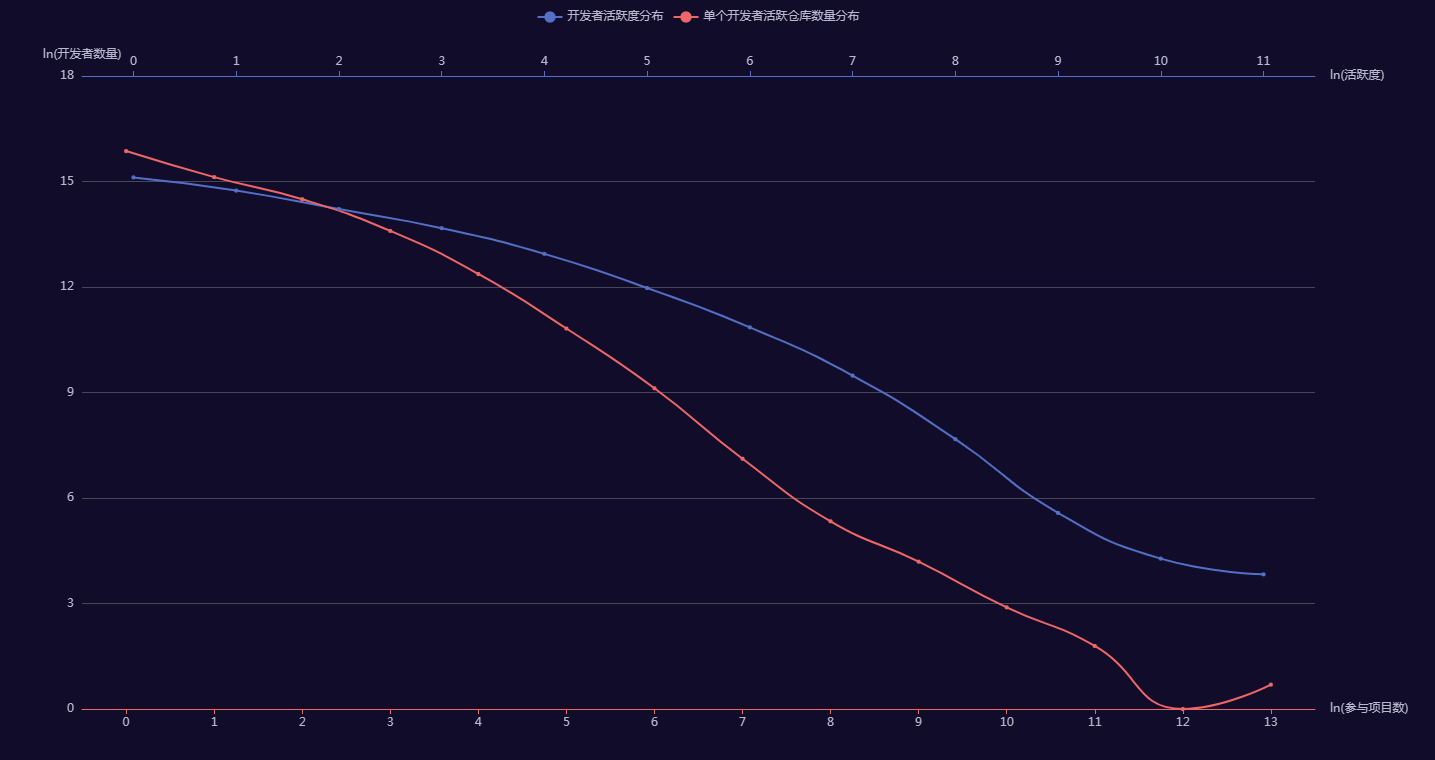
\includegraphics[width=130mm]{./figures/image2-1.png}
    \caption{开发者活跃度与活跃仓库数量分布图\\Figure 3-1: Distribution diagram of developer activity and the number of active warehouses}
\end{figure}

\par 图2-1使用双对数坐标系绘制,图上方的横坐标表示开发者活跃度,图下方横坐标表示开发者参与项目数量,纵坐标表示开发者数量,所谓双对数坐标,就是将原来的线性坐标轴都取自然对数,可以看到开发者活跃度与活跃仓库数量的分布符合幂律分布。经统计,活跃度超过 2,000 的开发者数量为 5,445 个,占全域开发者数量不足万分之六。而大部分开发者活跃度都在 [0, 500] 区间内,占全域开发者数量的 99.45\%,说明大多数开发者还是处于低活跃度的一个状态。观察曲线尾部,我们发现开发者活跃仓库数量在最后有一个回升,其实是由于部分未被过滤掉的自动化协作类账号的活跃仓库数量巨大,远超正常人类开发者,因此尾部形成V形曲线。

\par 由于开源开发者在地理位置上遍布全球,他们具有不同的工作时间分布情况。通过对Github事件日志的详细时间戳数据可视化,可以看到在UTC标准时间下,全球的开源开发者工作时间分布具有明显的规律,如图2-2所示,横轴为一天 24 个小时(UTC标准时间),纵轴为一周 7 天,圆点大小表示该时段项目内产生的日志量的总和。
\begin{figure}[H]
    \centering
    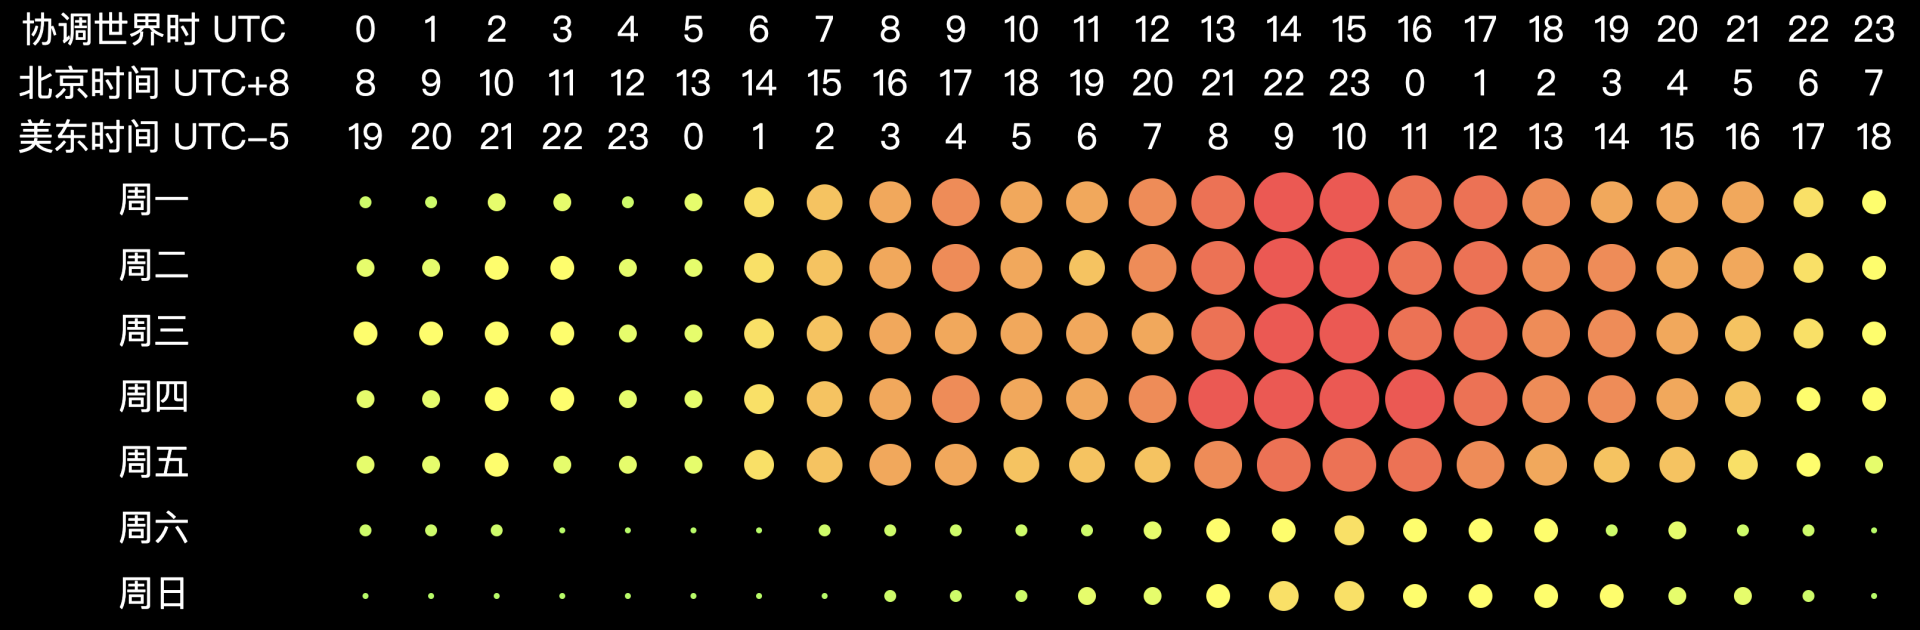
\includegraphics[width=130mm]{./figures/image2-2.png}
    \caption{GitHub 2020 年全球日志时间分布情况\\Figure 3-2: The global log time distribution of Github in 2020}
\end{figure}

\par 如果从日志中抽取每个开发者独立的日志在每日不同时间段的分布情况,并通过对开发者进行时区估计后将其移动合并到同一时区,就能够得到开源开发者的典型工作时间分布情况,从而推断出开发者所属时区、地区,或是根据项目成员的协作时间分布,来判断一个项目的国际化程度。如图2-3所示,对项目内部所有开发者进行时区估计,随后以UTC标准时间下的24个时区为横轴,以每个时区开发者比例为纵轴,作分布直方图。
\begin{figure}[H]
    \centering
    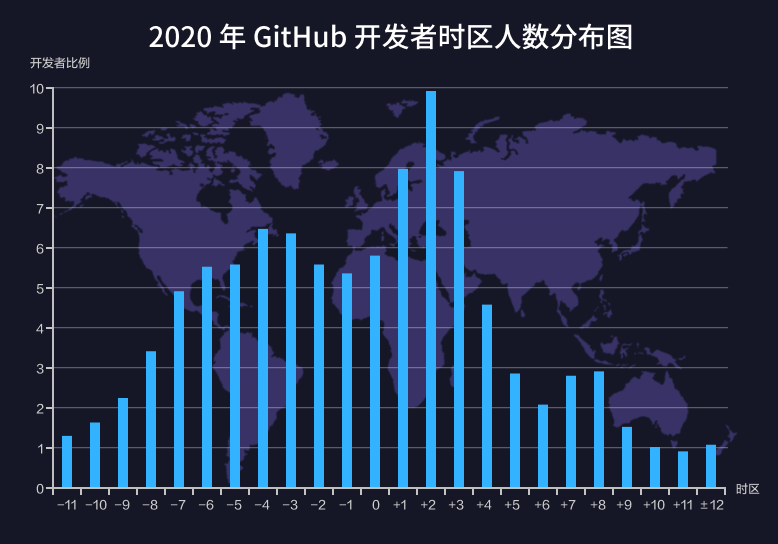
\includegraphics[width=90mm]{./figures/时区分布.png}
    \caption{GitHub 2020 年全球开发者时区人数分布图\\Figure 3-3: GitHub global developer time zone distribution map in 2020}
\end{figure}

\par 开发者的地理分布情况一直是开源项目全球化指标的一个重要方面,然而一直以来没有较好的方式来估计开发者所在时区,但在全域日志数据下,开发者的个人行为为我们提供了有效的估计手段。可以在全域范围或特定开发者群体内估计开发者在不同时区的占比情况,从而有效判断 GitHub 全域或特定项目内的全球化覆盖情况。

\par 另一方面,在不同的项目中,开源开发者们会使用不同的语言,也具有着一定的技术学习路线\cite{dabbish2012social},即主要使用的语言事件数量产生明显的增、减变化。在开源社区,由个体语言选择产生的变化组成了社区开发语言迭代的趋势,反之,开发语言的流行趋势也影响着开发者的学习路径。根据开源社区中活动频繁、贡献最大的一批用户的学习路径,就可以形成全域开发语言的流行趋势预测,从而为开发者的发展提供参考。
\begin{table}[htbp]\center
    \caption{GitHub 2020 年全域活跃开发者和 Top10 万活跃开发者语言分布对比\\ Table 3-1:  Comparison of the language distribution of GitHub's global active developers and the top 100,000 active developers in 2020}
    \begin{tabular}{|c|cc|cc|}
        \hline
        排名 & 全域开发者语言榜 & \makecell*[c]{全域范围\\开发者账号数} & \makecell*[c]{Top 10万开发者语言榜} &\makecell*[c]{Top 10万范围\\开发者账号数}\\
        \hline
        1 & JavaScript & 305,814 & JavaScript & 15,858 \\
        2 & Python & 175,610 & Python & 10,866 \\
        3 & HTML & 159,303 & TypeScript & 7,419 \\
        4 & Java & 139,673 & Java & 6,665 \\
        5 & Ruby & 87,780 & Go & 5,094 \\
        6 & TypeScript & 85,116 & C++ & 4,204 \\
        7 & C\# & 54,343 & Ruby & 3,802 \\
        8 & PHP & 52,915 & HTML & 3,490 \\
        9 & C++ & 47,799 & PHP & 3,000 \\
        10 & CSS & 46,428 & C\# & 2,892 \\
        \hline
    \end{tabular}
\end{table}
\par 将2020年全域所有活跃开发者使用的语言分布和活跃度 Top 10 万的开发者使用的语言分布情况进行对比,可以看到存在着一定的区别,如表3-1所示。

\begin{figure}[H]
    \centering
    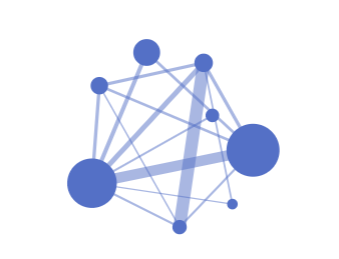
\includegraphics[width=80mm]{./figures/开发者协作网络图.png}
    \caption{某项目的开发者协作网络图\\Figure 3-4: The developer collaboration network diagram on a repository}
\end{figure}

\par 除了个体之间的差异,不同的开发者之间也存在着协作关系\cite{廖志芳2019github开源软件开发过程中关键用户行为分析}。在某一开源项目中,来自不同开发者的贡献使他们构成协作网络,如图3-4所示,对于在该项目中作出贡献的开发者,取top N位(N由用户定义配置)生成网络图,图中节点描述各开发者,节点大小描述开发者对该项目的贡献量,节点之间边的粗细描述两个开发者之间的协作活跃度\cite{thung2013network}。

\par 同一位开发者又有可能参与了多个项目,于是项目与项目之间也具有了关联性。综上两个方面考虑,优秀的开发者对项目具有着影响力,同时优秀项目更容易聚集优秀的开发者,这两者之间相互具有作用力。这样的关系可以用协作网络来进行可视化描述,通过项目协作关联度和社区发现算法对项目进行聚类,从而得到基于协作行为的聚类效果,并用于项目的大致分类。

\par 根据连通性分析,在全域约 105 万个开源项目中,共分成了 44,990 个连通子图,其中 935,231 个项目在协作关系下构成一个巨大连通子图,其他 44,989 个连通子图中最大的子图包含 200 个项目,最小的包含 1 个项目,包含了 100 个项目以上的连通子图仅 9 个。这意味着全域活跃项目中 89\% 的项目构成了一个巨大的协作网络,也就是 GitHub 开源世界的核心。而另外还有将近 4.5 万个小的协作孤岛,这些小的协作网络与开源世界不连通,意味着这些项目上的所有开发者都仅在自己的项目群中协作,从未在其他项目上有过活跃行为,同时在开源核心中的任意开发者也都没有在这个项目群中产生过协作行为\cite{刘玉辉2018github}。


